	\begin{figure}
		\centering
		\begin{subfigure}{0.4\textwidth}
			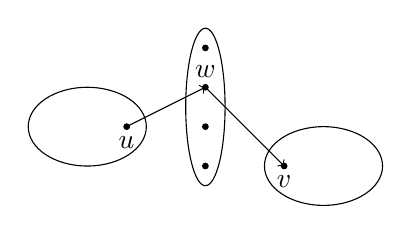
\begin{tikzpicture}[scale = 0.5]
			
			\filldraw (-1,2) circle (2pt) node[below] {$u$};    
			\filldraw (1,1) circle (2pt);    
			\filldraw (1,2) circle (2pt);    
			\filldraw (1,3) circle (2pt) node[above] {$w$};    
			\filldraw (1,4) circle (2pt);
			\filldraw (3,1) circle (2pt) node[below] {$v$};	
			
			\draw (-2,2) circle [x radius=1.5cm, y radius=10mm];		
			\draw[->] (-1,2) -- (1,3);
			
			\draw (4,1) circle [x radius=1.5cm, y radius=10mm];	
			\draw[->] (1,3) -- (3,1);
			
			\draw (1,2.5) circle [x radius=0.5cm, y radius=20mm];		
			
			
			\end{tikzpicture}
			
			\caption{\scriptsize The $s$-$t$ path takes a vertex of the separator}
			\label{fig:viaseparator}
			
		\end{subfigure}
	\hfill
		\begin{subfigure}{0.4\textwidth}
			\centering
			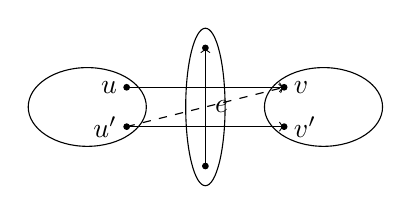
\begin{tikzpicture}[scale = 0.5]
			
			\filldraw (-1,2) circle (2pt) node[left] {$u'$};    
			\filldraw (1,1) circle (2pt) ;
			\filldraw (1,4) circle (2pt) ;
			\filldraw (3,2) circle (2pt) node[right] {$v'$};			
			
			\filldraw (-1,3) circle (2pt) node[left] {$u$};			
			\filldraw (3,3) circle (2pt) node[right] {$v$};			
			
			\draw[->] (-1,2) -- (3,2);
			
			\draw (-2,2.5) circle [x radius=1.5cm, y radius=10mm];
			\draw (1,2.5) circle [x radius=0.5cm, y radius=20mm];	
			\draw (4,2.5) circle [x radius=1.5cm, y radius=10mm];		
			
			
			\draw[->] (-1,3) -- (3,3);
			\draw[->] (1,1) --node[right] {$e$} (1,4) ;
			\draw[dashed, ->] (-1, 2) -- (3,3);  
			
			
			\end{tikzpicture}
			
			\caption{\scriptsize The $s$-$t$ path crosses an edge of the separator}
			\label{fig:viaedgecrossing}
		\end{subfigure}
		
		\caption{ }
		
	\end{figure}
